
\chapter{Quartiers et contrats}
\label{chap:quartiers}

\section{Objectifs}

La gestion des quartiers et des contrats constitue une partie importante de l'application AquaVolt. Elle permet d'organiser les abonnements des clients et de rattacher chaque consommation à un contrat précis.

Un client peut posséder plusieurs contrats associés à différents quartiers et types d'activité. Cette organisation permet de distinguer ses consommations et de faciliter leur suivi ainsi que leur facturation.

Les principaux objectifs de ce module sont :
\begin{itemize}
    \item gérer les quartiers selon leur type d'activité ;
    \item créer et consulter les contrats des clients ;
    \item permettre la résiliation d'un contrat actif ;
    \item associer chaque consommation à un contrat ;
    \item prendre en charge les clients possédant plusieurs contrats.
\end{itemize}

\section{Table quartier}

La table \texttt{quartier} permet de représenter les quartiers utilisés dans la gestion des contrats.

Elle contient les attributs suivants :
\begin{itemize}
    \item \texttt{id\_quartier} : identifiant unique du quartier ;
    \item \texttt{nom} : nom du quartier ;
    \item \texttt{type\_activite} : type d'activité associé au quartier ;
    \item \texttt{date\_creation} : date de création de l'enregistrement.
\end{itemize}

Le type d'activité peut prendre trois valeurs :
\begin{itemize}
    \item \texttt{RESIDENTIEL} ;
    \item \texttt{COMMERCIAL} ;
    \item \texttt{INDUSTRIEL}.
\end{itemize}

Une contrainte d'unicité est définie sur le couple
\texttt{(nom, type\_activite)}. Ainsi, un même nom de quartier peut être utilisé avec un type d'activité différent, mais le même couple nom-type ne peut pas être enregistré deux fois.

\section{Table contrat}

La table \texttt{contrat} représente les contrats établis entre les clients et le fournisseur. Chaque contrat est associé à un seul client et à un seul quartier.

Elle contient les attributs suivants :
\begin{itemize}
    \item \texttt{id\_contrat} : identifiant unique du contrat ;
    \item \texttt{id\_client} : référence du client concerné ;
    \item \texttt{id\_quartier} : référence du quartier associé ;
    \item \texttt{numero\_contrat} : numéro unique du contrat ;
    \item \texttt{date\_debut} : date de début du contrat ;
    \item \texttt{date\_fin} : date de fin éventuelle ;
    \item \texttt{statut} : état du contrat (\texttt{ACTIF} ou \texttt{RESILIE}) ;
    \item \texttt{date\_creation} : date de création de l'enregistrement.
\end{itemize}

Le numéro du contrat est unique. De plus, une contrainte vérifie que la date de fin, lorsqu'elle est renseignée, n'est pas antérieure à la date de début.

Les clés étrangères assurent le rattachement du contrat à un client et à un quartier existants.

\section{Gestion des quartiers}

La gestion des quartiers est réalisée à travers la classe \texttt{QuartierBD}, située dans le dossier \texttt{BD/}, et le contrôleur \texttt{Traitement/Quartier.php}.

La classe \texttt{QuartierBD} fournit les opérations suivantes :
\begin{itemize}
    \item \texttt{lister()} : récupérer la liste des quartiers ;
    \item \texttt{trouver()} : rechercher un quartier par son identifiant ;
    \item \texttt{existe()} : vérifier l'existence d'un quartier selon son nom et son type d'activité ;
    \item \texttt{creer()} : enregistrer un nouveau quartier.
\end{itemize}

Le contrôleur vérifie que l'utilisateur possède le rôle fournisseur et que les données soumises respectent les règles de validation. Il contrôle notamment que le nom est renseigné, que sa longueur ne dépasse pas 100 caractères et que le type d'activité appartient aux valeurs autorisées.

Avant la création, le système vérifie également qu'un quartier possédant le même nom et le même type d'activité n'existe pas déjà.

L'interface correspondante est disponible dans \texttt{IHM/quartier/index.php}. Elle permet d'ajouter un quartier et de consulter les quartiers enregistrés.

\section{Gestion des contrats}

La gestion des contrats repose sur la classe \texttt{ContratBD}, située dans \texttt{BD/Contrat.php}, et le contrôleur \texttt{Traitement/Contrat.php}.

La classe \texttt{ContratBD} permet notamment :
\begin{itemize}
    \item de lister les contrats d'un client ;
    \item de lister les contrats du fournisseur ;
    \item de rechercher un contrat par son identifiant ;
    \item de vérifier l'appartenance d'un contrat à un client ;
    \item de vérifier l'unicité du numéro de contrat ;
    \item de créer un nouveau contrat ;
    \item de résilier un contrat actif.
\end{itemize}

Lors de la création d'un contrat, le système vérifie que le client appartient au fournisseur connecté, que le numéro du contrat est renseigné et disponible, et que le quartier sélectionné existe.

Les dates sont également contrôlées. Si une date de fin est renseignée, elle ne doit pas être antérieure à la date de début.

Un nouveau contrat est créé avec le statut \texttt{ACTIF}. La résiliation est effectuée par une requête de type POST, après vérification du jeton CSRF et de l'appartenance du contrat au fournisseur connecté. Le statut passe alors à \texttt{RESILIE} et la date de fin est renseignée si elle ne l'était pas déjà.

L'interface \texttt{IHM/contrat/index.php} présente les contrats avec le numéro, le client, le CIN, le quartier, le type d'activité, les dates et le statut. Elle permet également de résilier les contrats actifs.

\section{Contrat par défaut et migration}

L'évolution du modèle de données a nécessité l'ajout de la gestion des contrats à une structure qui associait auparavant directement les consommations aux clients.

La migration \texttt{003\_quartier\_contrat.sql} réalise cette évolution en plusieurs étapes :

\begin{enumerate}
    \item création des tables \texttt{quartier} et \texttt{contrat} ;
    \item ajout de la colonne \texttt{id\_contrat} à la table \texttt{consommation}, initialement nullable ;
    \item création d'un quartier par défaut nommé \texttt{Non renseigné}, de type \texttt{RESIDENTIEL}, s'il n'existe pas ;
    \item création d'un contrat pour chaque client ne possédant aucun contrat, avec le numéro \texttt{CTR-} suivi de son identifiant et la date de début fixée au 1\textsuperscript{er} janvier 2026 ;
    \item rattachement des anciennes consommations au contrat correspondant à leur client ;
    \item modification de la colonne \texttt{id\_contrat} pour la rendre obligatoire ;
    \item remplacement de l'ancienne contrainte d'unicité par une contrainte portant sur le contrat et la période.
\end{enumerate}

Cette migration permet de conserver les anciennes données tout en adoptant le nouveau modèle de gestion multi-contrats.

Il convient de préciser que le contrat par défaut créé pendant cette migration sert à rattacher les anciennes données. La structure de la table \texttt{contrat} ne contient pas de colonne spécifique indiquant qu'un contrat est le contrat par défaut.

\section{Rattachement des consommations}

Chaque consommation est désormais associée à un contrat grâce à la colonne \texttt{id\_contrat} de la table \texttt{consommation}.

La classe \texttt{ConsommationBD} permet de récupérer les contrats actifs d'un client et de vérifier qu'un contrat sélectionné lui appartient.

Lors de l'enregistrement d'une consommation, le système :
\begin{itemize}
    \item récupère les contrats actifs du client connecté ;
    \item sélectionne automatiquement le contrat lorsqu'un seul contrat actif existe ;
    \item demande au client de choisir un contrat lorsqu'il en possède plusieurs ;
    \item vérifie que le contrat sélectionné appartient bien au client ;
    \item vérifie qu'aucune consommation n'existe déjà pour ce contrat et cette période.
\end{itemize}

La contrainte d'unicité définie sur
\texttt{(id\_contrat, periode\_mois, periode\_annee)}
empêche l'enregistrement de plusieurs consommations pour un même contrat durant une même période.

La consommation conserve ainsi un lien précis avec le contrat concerné, ce qui permet également de retrouver son historique et ses relevés précédents.

\section{Client avec plusieurs contrats}

L'application prend en charge le cas d'un client possédant plusieurs contrats associés à différents quartiers.

Lorsqu'un client possède un seul contrat actif, celui-ci est automatiquement sélectionné lors de l'enregistrement d'une consommation.

En revanche, lorsque plusieurs contrats actifs sont disponibles, le client doit choisir explicitement le contrat concerné. Ce choix est présenté dans le formulaire de saisie des consommations.

Le système vérifie ensuite que le contrat sélectionné appartient bien au client connecté et qu'il est actif.

Cette organisation permet de gérer séparément les consommations des différents contrats d'un même client et d'éviter leur confusion.

\section{Impact sur la facturation}

Le rattachement des consommations aux contrats permet d'assurer une facturation correspondant à chaque contrat.

Le service \texttt{FactureService}, situé dans \texttt{Traitement/FactureService.php}, reçoit l'identifiant d'une consommation pour générer sa facture.

Avant la création, il vérifie que la consommation existe et possède le statut \texttt{VALIDEE}. Il récupère ensuite les consommations calculées ainsi que les tarifs du fournisseur, puis utilise la classe \texttt{Tarification} pour calculer les montants.

La facture conserve notamment l'identifiant du client et celui de la consommation concernée. Elle ne possède pas de référence directe vers le contrat : le lien est établi indirectement à travers la consommation.

La génération de la facture et le changement du statut de la consommation vers \texttt{FACTUREE} sont exécutés dans une transaction. En cas d'erreur, les opérations sont annulées.

Enfin, une notification informe le client de la disponibilité de sa nouvelle facture.

\section{Tests}

Les scénarios suivants permettent de vérifier le bon fonctionnement du module des quartiers et des contrats :

\begin{longtable}{|p{0.8cm}|p{5cm}|p{5cm}|p{2cm}|}
\hline
\textbf{N\textsuperscript{o}} & \textbf{Scénario} & \textbf{Résultat attendu} & \textbf{Statut} \\
\hline
1 & Ajouter un quartier avec un nom et un type valides. & Le quartier est enregistré. & À vérifier \\
\hline
2 & Ajouter un quartier avec le même nom et le même type. & Le système refuse le doublon. & À vérifier \\
\hline
3 & Ajouter un quartier avec un type non autorisé. & Le système refuse les données invalides. & À vérifier \\
\hline
4 & Créer un contrat avec un client et un quartier existants. & Le contrat est créé avec le statut \texttt{ACTIF}. & À vérifier \\
\hline
5 & Créer un contrat avec un numéro déjà utilisé. & Le système refuse le numéro en double. & À vérifier \\
\hline
6 & Créer un contrat avec une date de fin antérieure à la date de début. & Le système refuse les dates invalides. & À vérifier \\
\hline
7 & Résilier un contrat actif. & Le statut devient \texttt{RESILIE}. & À vérifier \\
\hline
8 & Enregistrer une consommation avec un seul contrat actif. & Le contrat est automatiquement sélectionné. & À vérifier \\
\hline
9 & Enregistrer une consommation avec plusieurs contrats actifs. & Le client doit choisir le contrat concerné. & À vérifier \\
\hline
10 & Sélectionner le contrat d'un autre client. & Le système refuse l'opération. & À vérifier \\
\hline
11 & Enregistrer deux consommations pour le même contrat et la même période. & La contrainte d'unicité empêche le doublon. & À vérifier \\
\hline
\end{longtable}

Ces scénarios constituent une base de vérification fonctionnelle du module. Leur statut devra être actualisé en fonction des tests réellement exécutés.

\begin{figure}[H]
  \centering
  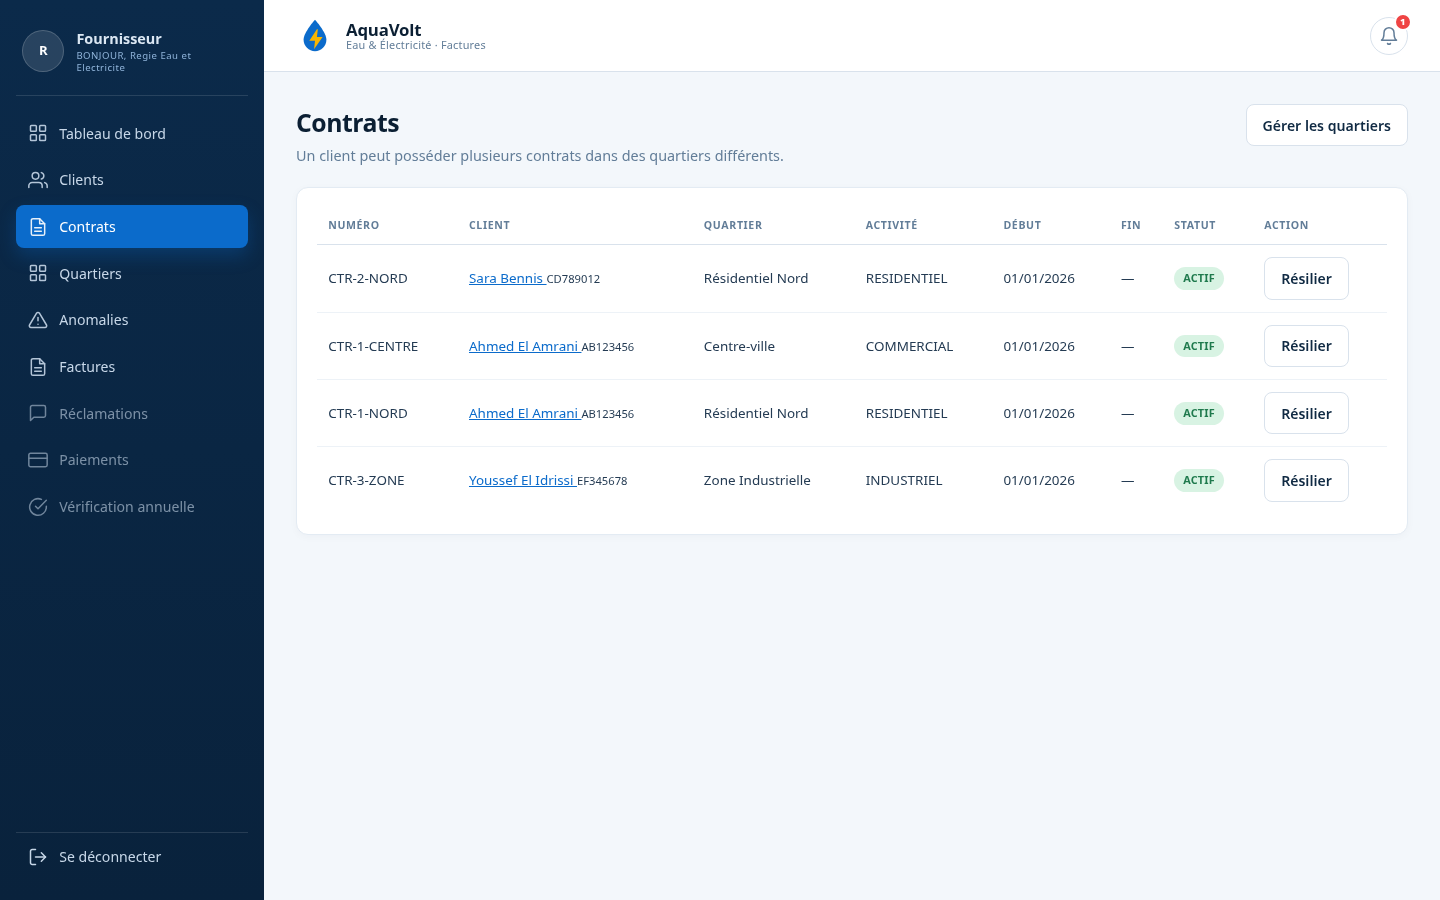
\includegraphics[width=0.92\textwidth]{../tests/screenshots/desktop/01_public_auth/14_contract_list.png}
  \caption{Liste des contrats du fournisseur}
  \label{fig:contrats}
\end{figure}

\begin{figure}[H]
  \centering
  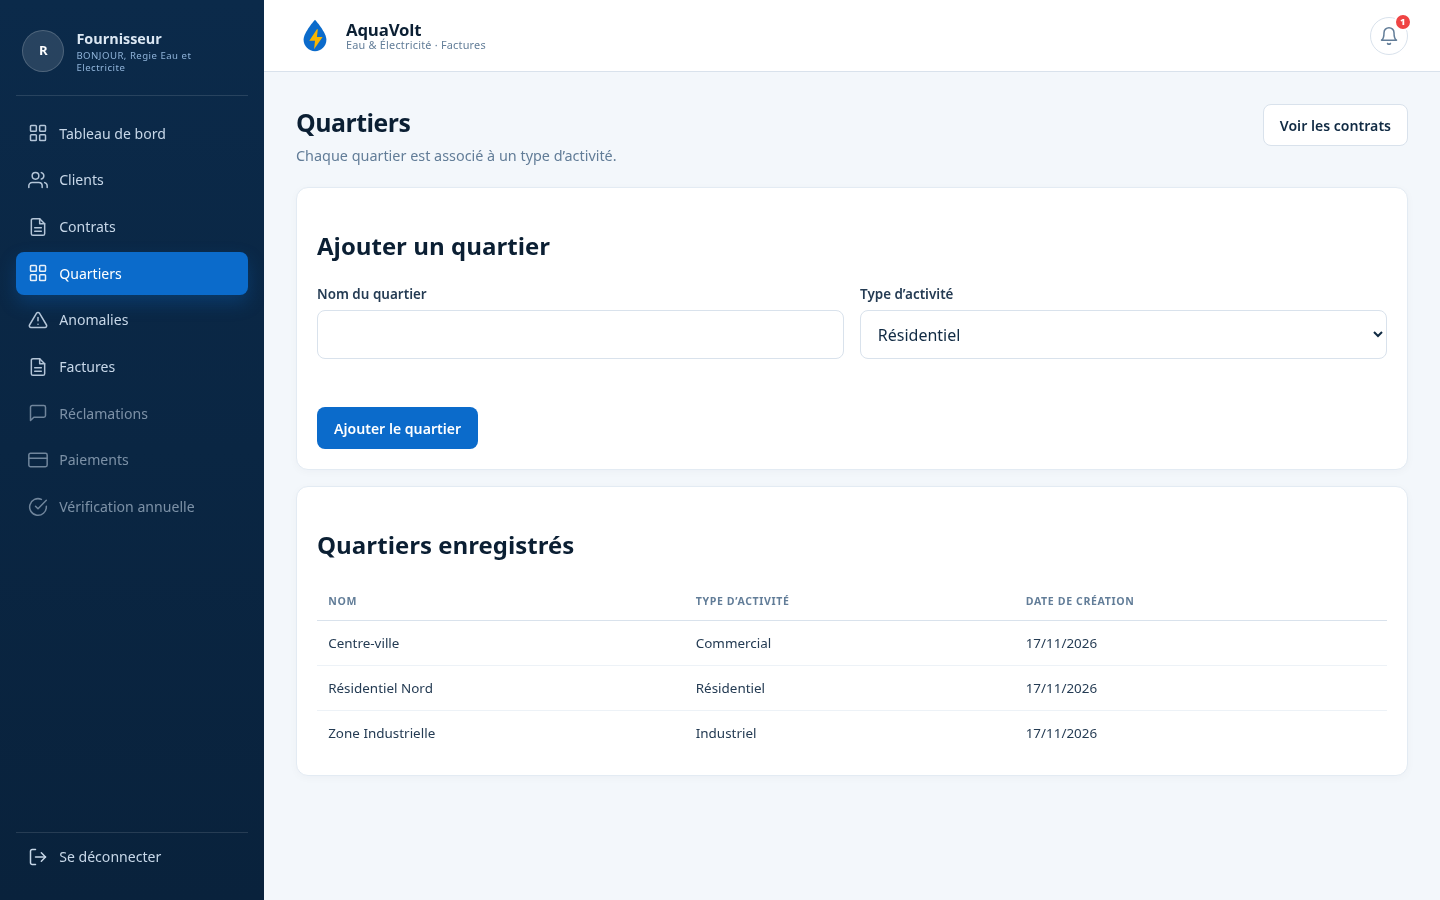
\includegraphics[width=0.92\textwidth]{../tests/screenshots/desktop/01_public_auth/11_quartier_list.png}
  \caption{Gestion des quartiers}
  \label{fig:quartiers}
\end{figure}
